\documentclass[../mcmpaper]{subfiles}
\begin{document}
	\section{Introduction}
	\subsection{Problem Background}
    While online marketplace is becoming more and more popular, the vast majority of people like shopping online. As the same time, everyone can give some text-messages(review) and star rating(1$\thicksim$5) for products they buy, these can provide some useful informations for potential customers. If this review provide unuseful information for potential customers, he/she can star rating for this review(helpfulness rating), these information is the most important part for online marketplace.
    \par
    Sunshine Company plan to introduce three new products in the online marketplace, and he wants to know about the above three indicators of microwave oven, a baby pacfier, and a hair dryer. They plan to hire a team to analyze the data given, and give some message about these:
    \begin{enumerate}[nosep, label=\textbullet]
        \item inform their online sales strategy.
        \item identify potentially important design features that would enhance product desirability. 
    \end{enumerate}
    \subsection{Restatements of the Problem}
    Considering the background information and restricted conditions identified in the problems statement, we need to solve the following problems.
    \begin{enumerate}[topsep=0pt, itemsep=0pt]
        \item According to the three product data set provieded, give the \label{item:1}
        \item According the analysis result of item~\ref{item:1}, you should solve these problems:
        \begin{enumerate}[nosep, ref=\theenumi(\theenumii)]
            \item  Identify data measures based on ratings and reviews that are most informative for Sunshine Company to track.\label{a}
            \item Identify and discuss time-based measures and patterns within each data set that might suggest that a product’s reputation is increasing or decreasing in the online marketplace.\label{b}
            \item Determine combinations of text-based measure(s) and ratings-based measures that best indicate a potentially successful or failing product.\label{c}
            \item Do specific star ratings incite more reviews? For example, are customers more likely to write some type of review after seeing a series of low star ratings?\label{d}
            \item Are specific quality descriptors of text-based reviews such as `enthusiastic', `disappointed', and others, strongly associated with rating levels?\label{e}
        \end{enumerate}
    \end{enumerate}
    \subsection{Our Work}
    Our workflow flow chart is shown in Figure~\ref{fig:1.3.1}, which systematically shows the method to solve the problem and the relationship between each step.
    \begin{figure}[!ht]
    \centering
    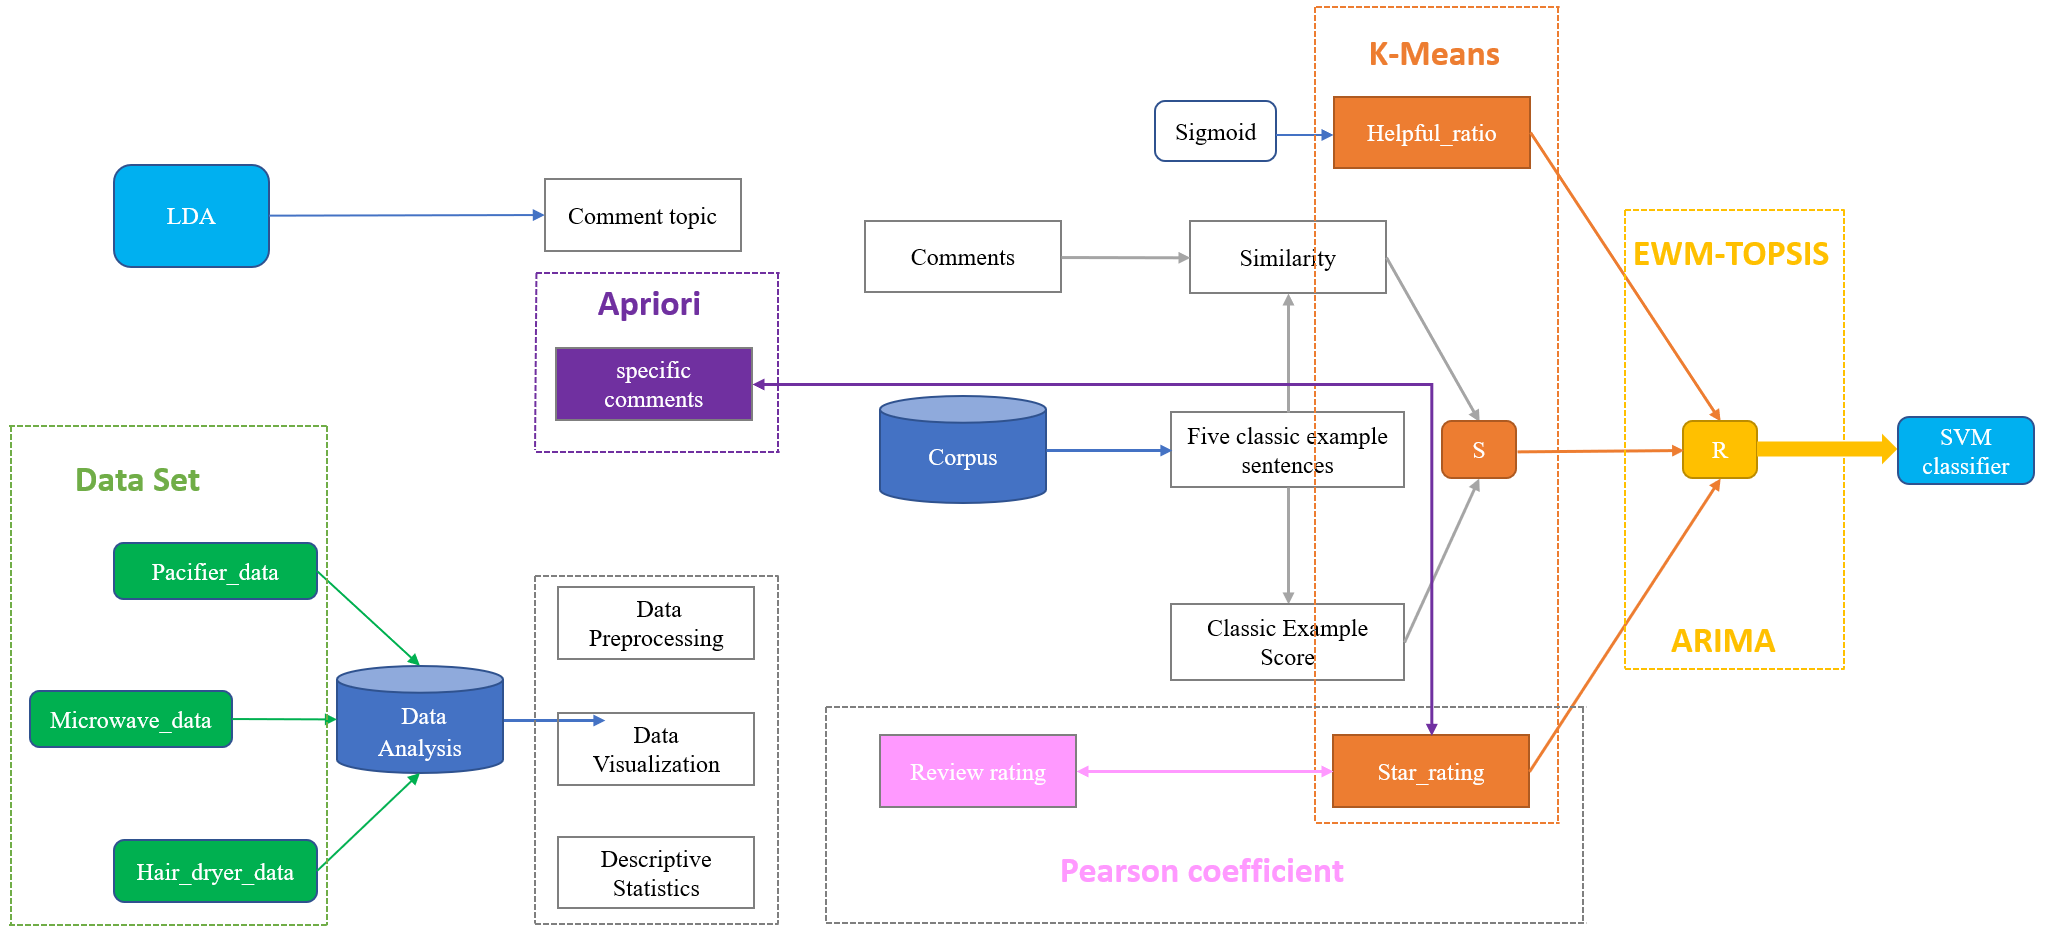
\includegraphics[scale=0.25]{1.3.1}
    \caption{Workflow}\label{fig:1.3.1}
    \end{figure}
    \par
    In Question 1, given three data sets are given, data analysis is carried out first. Comments with VINE N and verified\_purchase N are removed, review stars are visualized, and helpful\_ratio is constructed by sigmoid function. Description statistics for review stars and Helpful\_ratio. The LDA topic model is constructed to extract the topic of each comment, and the result is displayed as a word cloud.
    \par
    In Question~\ref{a}, the theme of effective comments is firstly used to construct 5 classic example sentences through self-built corpus, and the corresponding scores are set as 0.1, 0.3, 0.5, 0.7 and 0.9. Word2vec is used to analyze the similarity between the comments and the classic example sentences. The satisfaction rate of each comment is defined as the product of the score of the classic example with the greatest similarity and the maximum similarity. Then combining satisfaction rate, star rating and helpful\_ratio, k-means algorithm was used to classify customers' comments on products.
    \par
    For question~\ref{b}, the reputation rate R is defined, and the evaluation model of R is constructed through EWM-Topsis model, and the final score is R. Product review data has date attributes and is regarded as a time series. A prediction model of product reputation rate is constructed through ARIMA model for quantitative analysis.
    \par
    For question~\ref{c}, the One Class SVM model was first used to distinguish normal products from abnormal products (potentially successful or failed products), and then the SVM model was trained to give the judgment of successful or failed products.
    \par
    For question~\ref{d}, it is necessary to explore the correlation between review stars and reviews. Pearson correlation coefficient is used to explore the correlation between stars and the number of reviews, as well as between stars and review levels.
    \par
    For question~\ref{e}, the Apriori algorithm is used to mine frequent item sets and work out strong association rules between stars and specific comment words.
    \par
    Finally, we wrote a letter to the Marketing director of Sunshine Company, summarizing our analysis and results, and giving our own reasonable suggestions.
\end{document}
%%% Local Variables:
%%% mode: latex
%%% TeX-master: "../mcmpaper"
%%% End:
  